\documentclass{../exercisesheet}

\title{Datenkommunikation und Informationssysteme, Übung 1}
\author{
    Domenic Quirl \\ 354437
    \and
    Julian Schakib \\ 353889
    \and 
    Daniel Schleiz \\ 356092
}

\renewcommand{\Exercise}{Aufgabe}
\date{Übungsgruppe 14}

\usepackage{float}

\begin{document}
\maketitle
\pointtable

\begin{exercise}{1}
	Zum einen teilt der leitende Verpackungsingenieur die Ergebnisse der Befragung sowohl den Assistenten als auch der Rechtsabteilung mit, obwohl lediglich
	die Rechtsabteilung die unmittelbar darüber liegende Schicht wäre, die Assistenten befinden sich in der Schicht über der Rechtsabteilung. Da bei der vertikalen
	Kommunikation eine Schicht "übersprungen" wird und der Verpackungsingenieur sich nicht nur mit der Rechtsabteilung in Verbindung setzt, widerspricht dies
	dem \textit{ISO/OSI-Modell}. \\
	Zum anderen möchten die Geschäftsführungen und Assistenten Dinge vor Ort mit den Konstrukteuren und dem Braumeister klären, wobei die Schicht der	
	Rechtsabteilung übersprungen wird. Dies ist ebenfalls nicht konform mit dem \textit{ISO/OSI-Modell}. \\
\end{exercise}

\begin{exercise}{3}
	\begin{subexercise}
		Als Kommunikationspartner lassen sich der Wähler, welcher den Wahlzettel ausfüllt, und der Wahlvorstand, welcher den Wahlzettel zählt, identifizieren. Folgende
		Schichten der Kommunikation lassen sich dabei ausmachen (von "oben nach unten"):
		\begin{itemize}
		\item \textit{Bezirksschicht}, in welcher der Wahlzettel in der Urne für den Bezirk im blauen Umschlag liegt,
		\item \textit{Wahlamtsschicht}, in welcher der Brief im roten Umschlag geöffnet wird
		\item \textit{Postschicht}, in welcher der postale Versand des roten Umschlags stattfindet.
		\end{itemize}
		Es findet keine wirklich saubere Trennung der Schichten statt, da zum Beispiel der Wähler selbst seinen Wahlzettel mit PCIs versieht und direkt mit der Postschicht über
		den SAP Briefkasten vertikal kommuniziert anstatt mit der darunter liegenden Bezirksschicht, während erst auf der anderen Seite die Schichten wirklich durchlaufen werden.
	\end{subexercise}

	\begin{subexercise}
		Postschicht:
		\begin{itemize}
		\item \textit{PCI:} Aufdruck für die interne Verarbeitung auf der Schicht (geht nicht aus dem Text hervor)
		\item \textit{SDU:} Roter Briefumschlag mit Inhalt
		\item \textit{PDU:} Bedruckter Brief mit rotem Umschlag
		\end{itemize}
		Wahlamtsschicht:
		\begin{itemize}
		\item \textit{PCI:} Roter Umschlag (leer) und eidesstattliche Erklärung
		\item \textit{SDU:} Blauer Umschlag mit Inhalt
		\item \textit{PDU:} Geschlossener roter Umschlag mit Inhalt
		\end{itemize}
		Bezirksschicht:
		\begin{itemize}
		\item \textit{PCI:} Blauer Umschlag (leer)
		\item \textit{SDU:} Wahlzettel
		\item \textit{PDU:} Geschlossener blauer Umschlag mit Inhalt
		\end{itemize}
	\end{subexercise}
\end{exercise}


\begin{exercise}{5}
	\begin{subexercise}
	NRZI-M (mit Pegeln 1 und -1):
	\begin{figure}[H]
		\centering
  		\scalebox{.8}{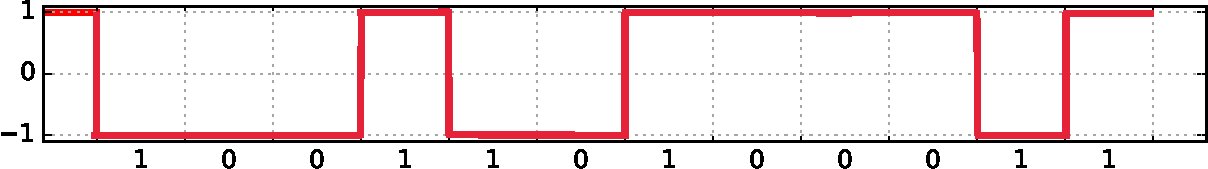
\includegraphics{2_2nrzi-m.pdf}}
	\end{figure}
	Unipolar RZ:
	\begin{figure}[H]
		\centering
  		\scalebox{.8}{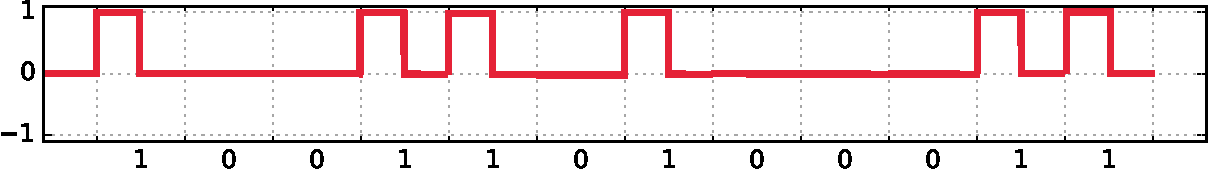
\includegraphics{2_2unipolar-rz.pdf}}
	\end{figure}
	Manchester:
	\begin{figure}[H]
		\centering
  		\scalebox{.8}{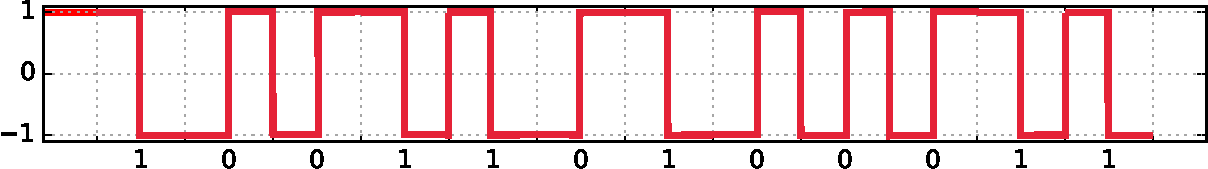
\includegraphics{2_2manchester.pdf}}
	\end{figure}
	Biphase-M:
	\begin{figure}[H]
		\centering
  		\scalebox{.8}{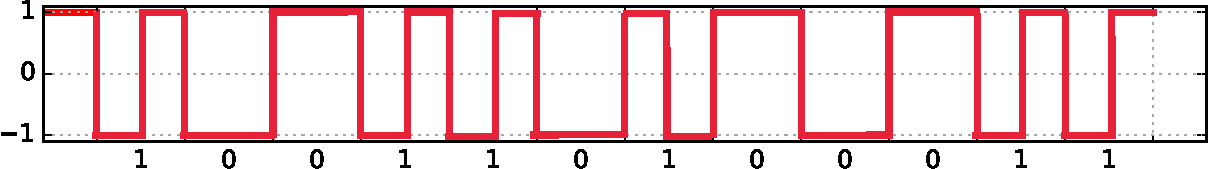
\includegraphics{2_2biphase-m.pdf}}
	\end{figure}
	RZ:
	\begin{figure}[H]
		\centering
  		\scalebox{.8}{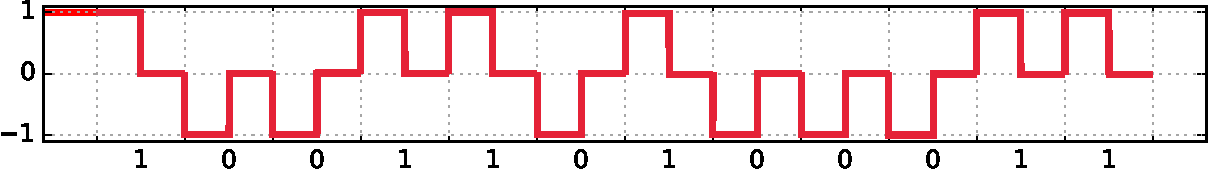
\includegraphics{2_2rz.pdf}}
	\end{figure}
	NRZ-L:
	\begin{figure}[H]
		\centering
  		\scalebox{.8}{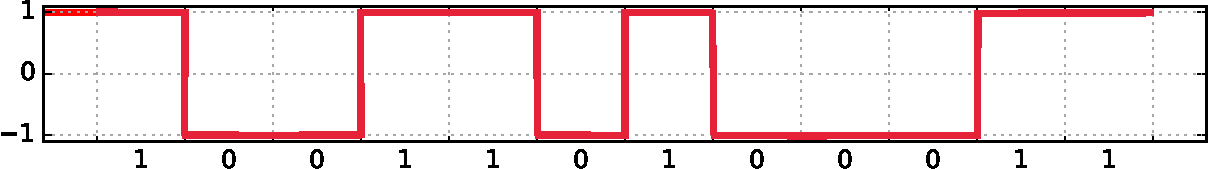
\includegraphics{2_2nrz-l.pdf}}
	\end{figure}\ \\
	\end{subexercise}

	\begin{subexercise}
	Mit 4B/5B Kodierung ergibt sich die Bitfolge 100111011010101 und die zu übertragende Signalfolge:
	\begin{figure}[H]
		\centering
  		\scalebox{.8}{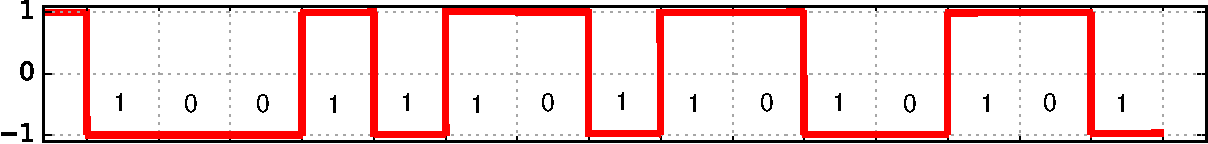
\includegraphics{2_2b.pdf}}
	\end{figure}
	\end{subexercise}

	\begin{subexercise} 
		Im Basisbandverfahren wird das gesamte Frequenzspektrum des Mediums genutzt. Dies ist für Ethernet durchaus sinnvoll, da es meist in lokalen Netzen
		eingesetzt wird, in welchen sich (relativ betrachtet) nicht so viele Kommunikationsteilnehmer befinden und es einfacher zu realisieren ist als ein Modulationsverfahren.\\
		Modulationsverfahren ergeben wiederum für DSL Sinn, da man potenziell viele Teilnehmer hat und man mittels Modulation Kanäle realisieren kann, indem man nur
		einen gewissen Teil der Bandbreite nutzt.
	\end{subexercise}
\end{exercise}

\begin{exercise}{1.5}
	\begin{subexercise}
	Ja, die Übertragungsgeschwindigkeit kann kleiner als die Schrittgeschwindigkeit sein. Dies ist zum Beispiel dann sinnvoll, wenn die langsamere Übertragungsgeschwindigkeit daher stammt, dass durch Leitungscodes wünschenswerte Eigenschaften wie Selbsttaktung oder die Vermeidung von Gleichstrom erzielt werden, der Code dafür aber zusätzliche Schritte benötigt. Ein konkretes Beispiel hierfür wäre die Übertragung eines binären Signals (eigentlich Übertragungsgeschwindigkeit = Schrittgeschwindigkeit) mittels eines RZ-Codes. Dieser ist selbsttaktend, benötigt aber zwei Schritte für die Übertragung eines Bits. Insgesamt wird also nur die halbe Übertragungsgeschwindigkeit erreicht.
	\end{subexercise}

	\begin{subexercise}
	Für den Datenaustausch müssen Sender und Empfänger synchronisiert sein. Deshalb muss ein Takt eingehalten werden, in dem in jedem Schritt ein Signal gesendet bzw. empfangen wird. Ein solches Signal kann zwar mehrwertig sein, also mehr als ein Bit codieren, jedoch sind die möglichen Signalwerte immer diskret, da sie ja eindeutig differenziert werden können müssen. Würde man unendlich viele Bits in einem solchen Signal codieren wollen, wären die diskreten Signalwerte unendlich nah beieinander und damit nicht mehr zu differenzieren.
	\end{subexercise}

	\begin{subexercise} 
	Die Schrittgeschwindigkeit kann deshalb nicht beliebig erhöht werden, weil auf einem gegebenen Trägermedium nur ein begrenztes Frequenzband genutzt werden kann, außerhalb dessen die Dämpfung durch das Medium eine Übertragung über eine gewisse Entfernung nicht mehr zulässt (Bandbreite). 
	\end{subexercise}
\end{exercise}

\begin{exercise}{4.5}
	\begin{subexercise}
		\begin{itemize}
			\item Kanal 1:
			\begin{itemize}
				\item $B = 20kHz - 5kHz=15kHz$
				\item $S/N=10^{3,1}\approx 1258,9$
				\item $R_{ny}=2*B*ld(n)=30.000*ld(n)$, bei einem zweiwertigen Signal $R_{ny} = 30.000 Bit/s$
				\item $R_{sh} = B*ld(1+S/N) \approx 15.000*ld(1+1258,9) \approx 154.486 Bit/s$
				\item $R_{max}=min\{R_{ny},R_{sh}\}\approx min\{30.000*ld(n), 154.486\}$
			\end{itemize}
			\item Kanal 2:
			\begin{itemize}
				\item $B = 40kHz - 22kHz=18kHz$
				\item $S/N=10^{2,5}\approx 316,23$
				\item $R_{ny}=2*B*ld(n)=36.000*ld(n)$, bei einem zweiwertigen Signal $R_{ny} = 36.000 Bit/s$
				\item $R_{sh} = B*ld(1+S/N) \approx 18.000*ld(1+316,23) \approx 149.569 Bit/s$
				\item $R_{max}=min\{R_{ny},R_{sh}\}\approx min\{36.000*ld(n), 149.569\}$
			\end{itemize}
			\item Kanal 3:
			\begin{itemize}
				\item $B = 95kHz - 74kHz=21kHz$
				\item $S/N=10^{2} = 100$
				\item $R_{ny}=2*B*ld(n)=42.000*ld(n)$, bei einem zweiwertigen Signal $R_{ny} = 42.000 Bit/s$
				\item $R_{sh} = B*ld(1+S/N) = 21.000*ld(1+100) \approx 139.822 Bit/s$
				\item $R_{max}=min\{R_{ny},R_{sh}\}\approx min\{42.000*ld(n), 139.822\}$
			\end{itemize}
		\end{itemize}	
	\end{subexercise}

	\begin{subexercise}
	Auf allen Kanälen liegt die durch 64-QAM theoretisch erreichbare Datenrate nach Nyquist oberhalb der maximalen Datenrate nach Shannon. Für Kanal 3 gilt dies zusätzlich auch für 16-QAM, da $42.000*ld(16)=168.000>139.822$. Kanal 3 kann also insgesamt maximal eine Datenrate von 139.822 Bit/s erreichen, mit 4-QAM sind es $42.000*ld(4)=84.000 Bit/s$. Kanal 2 kann hingegen 16-QAM in vollem Umfang nutzen, da $36.000*ld(16)=144.000<149.569$. Auf Kanal 2 kann also mittels 16-QAM eine Datenrate von 144.000 Bit/s erreicht werden. Kanal 1 erreicht aufgrund der geringeren Bandbreite nur $30.000*ld(16)=120.000 Bit/s$, was zwar ebenfalls unterhalb der 154.486 Bit/s nach Shannon liegt, aber langsamer ist als Kanal 2.
	
	Die maximale Datenrate erzielt also Kanal 2 bei der Verwendung von 16-QAM. Sie liegt bei 144.000 Bit/s.
	\end{subexercise}
\end{exercise}

\end{document}
